\documentclass[journal]{IEEEtran}
% IEEE Transactions on Industrial Informatics -- anonymous regular-paper draft
% Compile: latexmk -pdf main.tex
\usepackage{amsmath,amssymb,amsfonts}
\usepackage{algpseudocode}
% Local XeTeX/Tectonic builds: route IEEEtran's ptm (Times) family requests to
% the legacy Times Type1 faces so metrics match the pdfLaTeX reference build;
% the latexmk -pdf (pdfLaTeX) path is unaffected.
\usepackage{iftex}
\ifxetex
  \DeclareFontFamily{TU}{ptm}{}
  \DeclareFontShape{TU}{ptm}{m}{n}{<->ptmr8t}{}
  \DeclareFontShape{TU}{ptm}{b}{n}{<->ptmb8t}{}
  \DeclareFontShape{TU}{ptm}{m}{it}{<->ptmri8t}{}
  \DeclareFontShape{TU}{ptm}{b}{it}{<->ptmbi8t}{}
  \DeclareFontShape{TU}{ptm}{m}{sl}{<->ptmro8t}{}
  \DeclareFontShape{TU}{ptm}{m}{sc}{<->ptmr8t}{}
\fi
\usepackage{graphicx}
\usepackage{booktabs}
\usepackage{tabularx}
\usepackage{array}
\usepackage[table]{xcolor}
\usepackage{stfloats}
\usepackage{placeins}
\usepackage{url}
\urlstyle{same}
% Cross-references and citations. The cite package renders IEEE-style citation
% groups ([14]--[16], [20], [21]) with hyperref support.
\usepackage{cite}
\usepackage[colorlinks=true,linkcolor=black,citecolor=black,urlcolor=black]{hyperref}
\hypersetup{bookmarksnumbered=true,
  pdftitle={AgentWorkShop: A Modular Task-to-Device Integration Framework for Industrial Agents},
  pdfauthor={},
  pdfsubject={IEEE Transactions on Industrial Informatics},
  pdfkeywords={industrial informatics, industrial agents, multi-agent systems, production system integration, semantic data integration}}

% Float placement only; IEEEtran margins and body type remain unchanged.
\setcounter{topnumber}{4}
\setcounter{bottomnumber}{3}
\setcounter{totalnumber}{7}
\setcounter{dbltopnumber}{2}
\renewcommand{\topfraction}{0.95}
\renewcommand{\bottomfraction}{0.80}
\renewcommand{\textfraction}{0.03}
\renewcommand{\floatpagefraction}{0.72}
\renewcommand{\dbltopfraction}{0.95}
\renewcommand{\dblfloatpagefraction}{0.72}

% Tight but conventional float separation; body type and margins are unchanged.
\setlength{\textfloatsep}{8pt plus 2pt minus 3pt}
\setlength{\dbltextfloatsep}{8pt plus 2pt minus 3pt}
\setlength{\intextsep}{7pt plus 2pt minus 3pt}
\setlength{\abovecaptionskip}{3pt plus 1pt minus 1pt}
\setlength{\belowcaptionskip}{2pt plus 1pt minus 1pt}

\newcommand{\system}{the platform}
% Review copy is anonymous. The AI-use statement is maintained in
% AI-DISCLOSURE.md for the journal-approved disclosure channel and is not
% compiled into this manuscript.
\newif\ifblindreview
\blindreviewtrue

\begin{document}
\bstctlcite{IEEEbstctl}

\title{AgentWorkShop: A Modular Task-to-Device Integration Framework for Industrial Agents}

\author{}
\markboth{IEEE Transactions on Industrial Informatics, Submitted Manuscript}{AgentWorkShop: Task-to-Device Integration}

\maketitle

\begin{abstract}
Industrial agents must adapt to scene-specific process signals and protocols
while preserving links among task context, device commands, and process
evidence. This paper presents AgentWorkShop, a modular task-to-device framework
that composes task adapters, production context, shared named operations,
semantic input/output (I/O), runtime checks, configured drivers, and
service-owned records.
Registered tasks enter through the collaboration runtime, whereas direct
operation calls use the same dispatcher without creating a task. For writes,
applicable guards, any configured approval, and context revalidation precede
software dispatch; command receipts remain distinct from later process
observations.
We evaluate three caller routes---registered harness, fixture-backed
command-line task, and direct Representational State Transfer (REST)---across
cast-film and annealing simulators with different signal and protocol
mappings. Within the registered-harness route, deterministic fixed-request
replays isolate route execution from model selection. Six model-mediated
registered tasks and six deterministic executions across fixed-request
harness replays, direct REST calls, and fixture-backed command-line tasks
preserved their applicable record links; all 12 post-operation samples remained below their
scene target bands. A mock-state context guard rejected every injected
stale-context change before writes, while its ablation allowed six product/run
changes. One coating-line blueprint replay confirmed a simulator write. Four
deterministic simulator missions, one per scenario, ended within their
scenario-specific target windows. These results characterize selected
integration paths and scenario-specific simulator behavior; they do not
demonstrate process improvement or general portability.
\end{abstract}

\begin{IEEEkeywords}
Industrial agents, industrial communication, industrial informatics,
production systems, semantic data integration.
\end{IEEEkeywords}

\IEEEpeerreviewmaketitle

\section{Introduction}
\IEEEPARstart{I}{ndustrial-agent} deployments must connect each task to its
production context, process signals, and equipment interfaces. Prior work
studies end-to-end automation, control-sequence generation, modular factory
skills, and robotic-line control
\cite{xia2025control,huang2026made,koehle2026llmdriven,waseem2026pretrained},
as well as programmable logic controller (PLC) code generation,
context-aware control, resource discovery, shop-floor coordination,
digital-twin fault handling, and natural-language machine access
\cite{liu2026agents4plc,wu2025instructmpc,lim2025llmenabled,zhao2026shopfloor,gill2025llmdt,hofmann2025nlc}.
Recent systems add Asset Administration Shell (AAS)-grounded OPC Unified
Architecture (OPC UA) actions with signed approval, process and
instrumentation diagram (P\&ID)-grounded proposal checks, or governed
sensor--manufacturing execution system (MES)--enterprise resource planning
(ERP) evidence streams
\cite{graul2026aas,schall2026safe,lin2026agentic}. Across production lines,
agent roles, signal maps, protocols, objectives, and product/run context vary.
This paper examines a software-integration requirement at that boundary:
task routes and direct tool callers should share a named operation handler
while retaining route-appropriate evidence. Task routes can link task,
approval, command receipt, and process observation; direct calls retain
operation records without creating a task. We implement and evaluate this
contract without claiming that equivalent behavior is absent from prior
platforms.

We examine cast-film thickness control and annealing-zone temperature control,
which use different signals and interfaces but share a task-to-device path.
Each task needs production context, typed data-acquisition (DAQ) signals,
manufacturing execution system (MES) data, and a configured route from a named
operation to a device protocol. Fig.~\ref{fig:control-path} summarizes this
path: the goal and active context inform an operation proposal; shared checks,
route guards, any configured approval, and a pre-dispatch context recheck
govern writes through the DCW write-control subsystem. A command receipt
remains distinct from the later process observation. The evaluation covers
two simulator mappings and a documented coating-line onboarding replay.

\begin{figure}[!b]
\centering
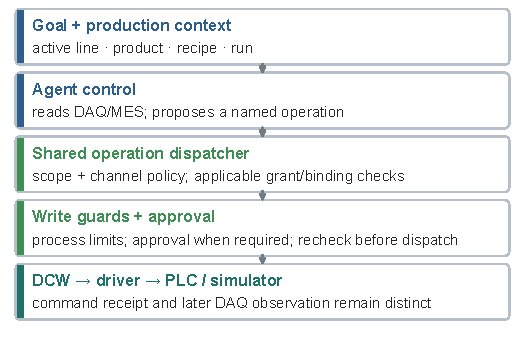
\includegraphics[width=\columnwidth]{resources/fig-agent-control.pdf}
\caption{Agent-control path for a configured industrial task. The agent uses
DAQ/MES context, passes shared operation checks, and routes writes through
process guards, conditional approval, and a pre-dispatch context recheck. DCW
and configured drivers provide device access; command receipts and later
process observations remain separate. The framework does not prescribe an
optimization policy.}
\label{fig:control-path}
\end{figure}

AgentWorkShop implements this path as a modular task-to-device framework.
Registered harnesses connect collaborative tasks to production context, MES
data, analysis and modeling services, DAQ/DCW nodes, and protocol-specific
drivers. Command-line, web, software development kit (SDK), Representational
State Transfer (REST), Model Context Protocol (MCP), and Agent-to-Agent (A2A)
interfaces serve different callers. Task and chat requests enter the
collaboration runtime; direct REST calls reach the shared dispatcher without
creating a task. Scene blueprints define signal maps, objectives, and guards,
while channel profiles, tool policies, and agent bindings scope operations.
The framework supplies this execution path without selecting routes
autonomously or prescribing an optimization strategy. Fig.~\ref{fig:arch}
shows the architecture, and Fig.~\ref{fig:runtime} traces a task through it.

The route study covers three caller routes---registered harness,
fixture-backed command-line task, and direct REST---across the two simulator
mappings. Within the registered-harness route, a fixed-request replay
separates route execution from model selection. A mock-state experiment tests
the approval-bound context check before software dispatch. A separate replay
onboards one documented coating-line blueprint with Modbus TCP and MES REST
interfaces. Four additional simulator scenarios record deterministic
operation calls and process responses for injection molding, wastewater
treatment, annealing, and biaxially oriented polyethylene terephthalate
(BOPET) film. The evidence is limited to these selected paths, one onboarding
configuration, and four scenario-specific control sequences.

This paper makes two contributions. First, it implements a modular execution
path that combines scene configuration, harness adapters, named operations,
shared checks, configured drivers, and service-owned records. For approved
recipe actions, approval is bound to the active line--product--recipe--run
tuple and rechecked just before software dispatch; this check is not an atomic
lock across device I/O. Second, it evaluates route-specific record continuity
for registered-harness tasks under model-mediated and fixed-request
conditions, fixture-backed command-line tasks, and direct REST calls across
two simulator mappings. It also reports four scenario-specific missions, one
coating-line onboarding replay, and a mock-state guard and ablation. Process
readings are reported separately from route-integration outcomes.

Section~II reviews related work. Section~III presents the design rationale,
architecture, and execution flow; Section~IV describes module functions and
integration. Section~V reports the experimental protocol and results,
Section~VI discusses evidence limits, and Section~VII concludes the paper.

\section{Related Work}
\label{sec:related}
This section relates AgentWorkShop to plant-facing industrial agents and to
production abstractions for context, tool access, and operational constraints.
Table~\ref{tab:nearest} compares two aspects of the integration contract:
whether task and direct-operation entries share a named handler, and how
operational evidence is associated. Entries describe reported features;
``not reported'' does not imply absence, and evaluation descriptions retain
each source's metrics.

\subsection{Industrial Agents and Plant Integration}
Industrial-agent systems, including large language model (LLM)-based systems,
span end-to-end automation control, supervisory
services, programmable logic controller (PLC) interfaces, manufacturing
coordination, and operator-facing machine access. Xia et al. present an
LLM agent framework for end-to-end industrial automation control, using
structured prompts and event-driven context for production planning and
operation \cite{xia2025control}. Huang et al. present a multimodal
architecture whose stated focus is automated control generation for
industrial cyber-physical systems \cite{huang2026made}. Biskupovic et al.
study agent-based supervision for service-oriented industrial systems
\cite{biskupovic2025supervision};
Agents4PLC and InstructMPC address PLC code generation and human--LLM
context-aware control, respectively
\cite{liu2026agents4plc,wu2025instructmpc}. Manufacturing studies consider
dynamic resource-capability exploration \cite{lim2025llmenabled}, multi-agent
shop-floor coordination \cite{zhao2026shopfloor}, and digital-twin-supported
fault handling \cite{gill2025llmdt}. Natural-language machine access
\cite{hofmann2025nlc} and real-time LLM control of a robot-operated serial
line \cite{waseem2026pretrained} extend this work to operator interfaces and
robotic-line control. Together, these studies address different operational
contexts, interfaces, and allocations of responsibility between agents,
operators, and controllers.

The closest architecture-level comparison is Xia et al., who connect cognitive,
digital-twin, and physical-automation layers and organize twin information as
state snapshots, event messages, and plan sequences
\cite{xia2025architecture}. Other nearby designs expose factory-module
operations through MCP with state-based tool filtering, constrain
manufacturing plans, or compose semantic recipes from OPC UA skills
\cite{koehle2026llmdriven,silva2025mcpmanufacturing,koehle2025semanticrecipes}.
Several recent systems also combine agent execution with approval, industrial
data, or audit records. Graul et al. ground proposals in the Asset
Administration Shell (AAS) and route approved actions through OPC UA Methods,
with signed approvals and audit logging \cite{graul2026aas}. Schall separates
advisory language-model agents from process and instrumentation diagram
(P\&ID)-grounded verification and execution, and evaluates structural checks
across five simulated process scenarios \cite{schall2026safe}; its context
includes supervisory control and data acquisition (SCADA) and standard
operating procedure (SOP) information. Lin and Chen build a governed
sensor--MES--ERP digital thread for closed-loop monitoring and control on real
manufacturing records \cite{lin2026agentic}. These works address
asset-specific approval, process validation, or closed-loop analytics. The
complementary question here is whether a modular task-to-device implementation
can route registered-harness and command-line task paths and a direct caller
through a shared named handler while preserving the records applicable to each
route; its approved recipe path also rechecks the
line--product--recipe--run tuple before software dispatch. The route study
examines two preconfigured simulator mappings, and a separate blueprint replay
checks one documented coating-line onboarding workflow through the existing
interfaces. Table~\ref{tab:nearest} positions these mechanisms by reported
features rather than comparative performance.
\begin{table*}[!t]
\centering
\caption{Reported shared-entry handling and evidence structure in selected
plant-facing studies. Shared handling means that task and direct-operation
entries resolve to the same named handler; ``not reported'' is not a claim
that a system lacks the feature. Evaluations retain source-specific scope and criteria.}
\label{tab:nearest}
\small
\setlength{\tabcolsep}{3pt}
\begin{tabularx}{\textwidth}{@{}>{\raggedright\arraybackslash}p{1.45cm}>{\raggedright\arraybackslash}p{2.6cm}>{\raggedright\arraybackslash}p{5.1cm}>{\raggedright\arraybackslash}X@{}}
\toprule
System & Shared handler for task and direct entries & Reported operation and evidence structure & Reported evaluation \\
\midrule
Xia et al. \cite{xia2025architecture} & Not reported & Cognitive, twin, and physical layers; twin snapshots, event messages, and plan sequences & Robotic automation and process-simulation cases \\
K{\"o}hle et al. \cite{koehle2026llmdriven} & Not reported & Injected live state and state-based filtering; MCP-to-OPC UA operations and MQTT coordination & Nine simulated production challenges \\
Vieira da Silva et al. \cite{silva2025mcpmanufacturing} & Not reported & Constrained multi-step plans over MCP manufacturing functions & Laboratory multi-step process \\
K{\"o}hle et al. \cite{koehle2025semanticrecipes} & Not reported & Semantic recipes composed from OPC UA skills; virtual commissioning & Unity assembly-workstation proof of concept \\
Graul et al. \cite{graul2026aas} & Not reported & AAS-grounded proposals, signed human approval, PLC-validated OPC UA Methods, and immutable audit log & Two laboratory PoCs; single scripted runs \\
Schall \cite{schall2026safe} & Not reported & P\&ID-, SCADA-, and SOP-grounded proposal verification with gated execution & Five simulated scenarios; 43 proposals and 50 LLM runs \\
Lin and Chen \cite{lin2026agentic} & Not reported & Governed sensor--MES--ERP digital thread with SOP-, risk-, and capability-aware action gating & 25,275 real records; operational metrics \\
\midrule
This work & Implemented; selected routes tested & Shared named dispatcher; task, approval, receipt, and sample links on task routes; receipts, readbacks, and run-tagged samples for direct calls & Two simulator mappings; one coating-line blueprint onboarding replay; context-guard test and ablation \\
\bottomrule
\end{tabularx}
\end{table*}

The operation checks complement safety-aware decision support
\cite{jiang2026agentic} but do not replace independent process protection.

\subsection{Production Context, Agent Interfaces, and Automation}
Industrial integration also depends on abstractions that are not specific to
agent architectures. The Model Context Protocol (MCP) specifies interoperable
tool discovery and call mechanisms \cite{mcp2024}; the operation-level scope,
policy, grant, and binding checks discussed here are AgentWorkShop's own
dispatcher rules, distinct from MCP transport authorization. In parallel,
ISA-88 and ISA-95 describe recipes and production operations
\cite{isa88_2010,isa95_2025}. Run-to-run methods connect process observations
to successive production runs \cite{moyne2000r2r}. At the agent level,
AgentSpec and CaMeL address tool behavior and capability-based information
flow \cite{wang2025agentspec,debenedetti2025camel}. Together, these standards
and agent-level mechanisms provide abstractions for production context, tool
interaction, and information flow. They motivate a focused implementation
question for this study: can a modular task runtime and direct-operation
interface converge on one named handler while preserving route-specific
evidence under scene-specific signal and protocol mappings? AgentWorkShop
implements this composition, and Section~V evaluates selected paths across
two configured simulator scenes and one separate blueprint replay. The
evaluation concerns integration behavior; it does not claim comparative
platform performance or general plant portability.

\section{System Design}
\label{sec:design}
AgentWorkShop is designed for industrial tasks whose agents, production
contexts, interfaces, and process signals vary between deployments. Its
architecture organizes these variations around shared task and operation
services, checks each proposed operation against the active production
context before device routing, and retains route-specific evidence that
distinguishes a command receipt from a measured process response.

\begin{figure*}[!t]
\centering
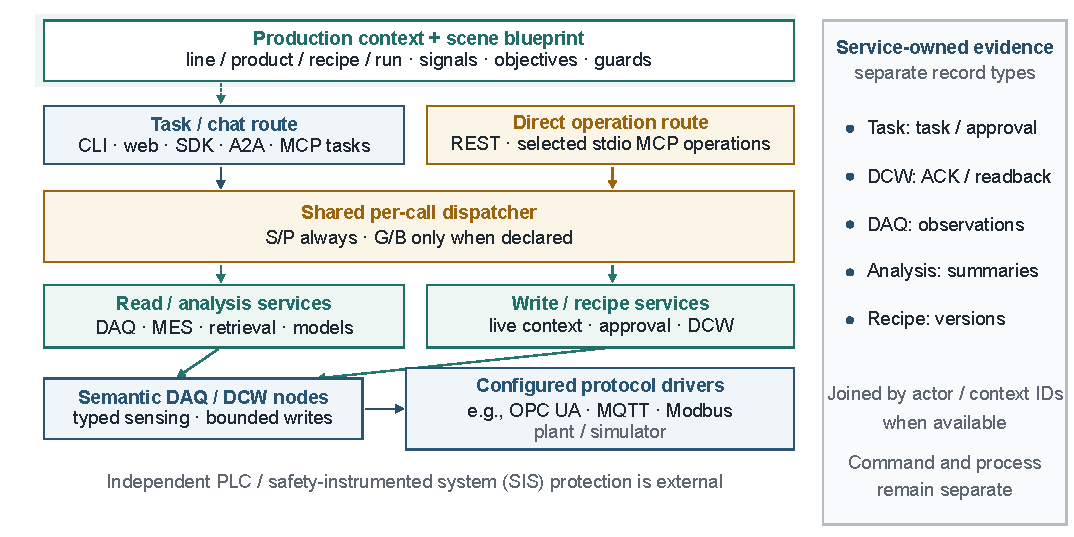
\includegraphics[width=\textwidth]{resources/fig-architecture-2026-9pt.pdf}
\caption{Architecture and record ownership. Task/chat routes enter the
collaboration runtime; direct REST and stdio-MCP calls enter shared dispatch
checks without creating a task. One dashed link marks configuration. Write
routes add approval and interval admission; recipe dispatch omits the
previous-recipe window. The shared dispatcher always
checks scope and channel policy, with grant and resource-binding checks applied
when required by the operation. Owning services retain distinct records. Only
REST was evaluated; stdio-MCP is shown but untested. Independent PLC and
safety-instrumented protection is external.}
\label{fig:arch}
\end{figure*}

\subsection{Design Rationale and Requirements}
\label{sec:principles}
Five requirements---scene variability, harness variability, operation
authority, outcome observability, and extensibility---organize six design
rules (D1--D6). These are deployment constraints drawn from the target
workflows. D1 stores scene settings as versioned data;
D2 provides registered harness, tool, and driver interfaces; D3 separates
proposal from execution; D4 treats the tool catalog as discovery rather than
permission; D5 routes actuator writes through the common DCW admission point;
and D6 retains evidence by operation.

The requirements trace to implementation as follows.
Scene variability maps to D1, scene blueprints, and context resolution;
harness variability and extensibility map to D2, the registered harness and
driver interfaces; operation authority maps to D3--D5, the shared dispatcher,
grants, bindings, and write admission; outcome observability maps to D6,
route-specific receipts, and observations. These interfaces are design
extension points; Section~\ref{sec:eval} tests selected task and direct-operation
routes and one documented blueprint-onboarding workflow. AgentWorkShop supplies
task and operation services;
agent strategy and independent process protection remain outside this design.

\subsection{Layered Architecture}
\label{sec:layers}
\label{sec:arch}
Fig.~\ref{fig:arch} summarizes the access routes, shared dispatch path,
production services, semantic I/O, configured drivers, and service ownership
of records. Task and chat routes enter the
collaboration band, which contains workspaces, channels, task queues, shared
memory, mailboxes, task templates, and harness adapters. A \emph{task route}
is an execution path through this runtime; a \emph{harness adapter} connects
an agent engine to its task execution interface. Direct REST tool
calls and the stdio MCP operation bridge bypass task execution in that band
(the upper-right direct-operation entry in
Fig.~\ref{fig:arch}) and enter the shared governance block without creating a
task or starting a harness turn; MCP management and task methods remain on
their service routes. Direct calls resolve current route state at invocation,
without an agent-turn prompt or a task record.
The governance block projects the operation catalog and applies the per-call
checks; write routes add the approval card and the admission interval. The
context block supplies the active line--product--recipe--run tuple to the gate
and scene maps, objectives, and guards to the handlers. The dashed link from
that block in Fig.~\ref{fig:arch} marks this configuration relationship; the
runtime assembles prompt-time context from the same records. The service band,
behind a route-handler interface that selects an adapter, provides
acquisition, write control, analysis, retrieval, and optional model services.
Field I/O resolves semantic nodes to built-in or plugin drivers for a plant or
simulator.

Each band has a distinct responsibility: task/chat routes enter the task
runtime, direct operations enter the dispatcher, and both use shared operation
checks. A harness adapter supplies agent-specific interaction, semantic nodes
hide protocol details, and the driver registry provides the device-facing
extension point. Owning services retain task, command, observation, and
version records separately and link them to actor and production context; no
single status conflates these outcomes.

\subsection{Cross-Module Execution Flow}
\label{sec:executionflow}
Fig.~\ref{fig:runtime} summarizes a task turn from entry through operation
execution, with route-specific evidence retained by owning services. Registered
harness adapters receive a scoped tool catalog during setup and supported
registry refreshes; the runtime assembles prompt-time production context for
each agent turn. This context is grounding information, not a task-pinned
transaction. For each returned tool call, the shared dispatcher rechecks
invocation scope and channel policy and, for industrial operations, current
grant and binding conditions before handler selection. The selected handler
then applies route-specific guards, active-run checks, approval
revalidation, and device-I/O steps as applicable. Command receipts and later
process observations remain distinct records.

For an industrial operation $u$ by agent $a$ in channel $c$, define the
shared dispatch condition as
\begin{equation}
\mathcal{A}(a,c,u)=\bigwedge_{X\in\mathcal{C}(u)}X(a,c,u),
\label{eq:dispatch-contract}
\end{equation}
where $S$, $P$, $G$, and $B$ denote invocation scope, current channel policy,
runtime grant, and the agent's binding to referenced resources, respectively.
$\mathcal{C}(u)\subseteq\{S,P,G,B\}$ is the set of predicates declared for
operation $u$; it always contains $S$ and $P$. The grant predicate $G$ is
omitted only for an explicitly grant-exempt industrial tool, and $B$ is
included when the operation declares resource references. A declared
no-reference operation omits $B$. Each included check must pass before
handler selection. The policy predicate includes channel tool selection,
profile, and duty-separation checks where configured. This condition is
necessary for handler selection, not sufficient for actuation: the selected
route applies its own guards and approval, then rechecks authority, context,
and applicable limits before dispatch.

For direct REST invocation, the API establishes $a$ and $c$ before applying
these checks. An agent token must match the requested agent identifier;
otherwise, an authenticated user must be the channel owner or an administrator.
The manager loads the channel-agent record to obtain the agent identity,
role, and channel, then rechecks invocation scope and channel tool policy.
Industrial operations continue through the declared shared grant and binding
checks.
Handlers resolve live production state from request identifiers and owning
services, supplying the authorization and production context for direct dispatch.

Fig.~\ref{fig:execution} gives reference pseudocode for the registered-harness
task path, not one literal orchestrator function. Direct REST tool invocation
bypasses the task runtime and harness but enters the same shared dispatcher.
Route-specific timing, approval, and evidence rules are detailed in
Section~\ref{sec:modules}.

\begin{figure*}[!t]
\centering
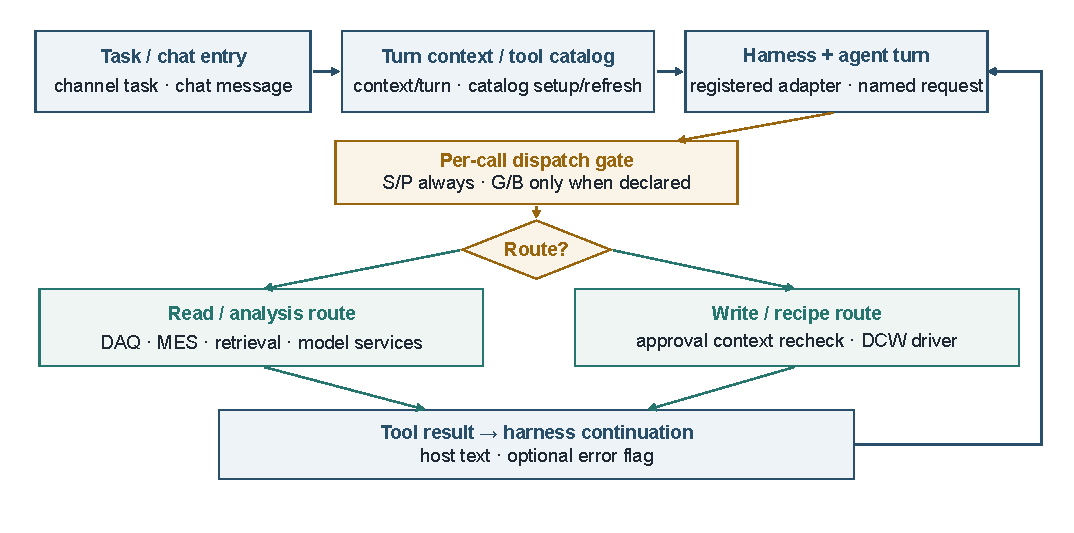
\includegraphics[width=\textwidth]{resources/fig-runtime-2026-9pt.pdf}
\caption{Registered-harness task flow. The runtime invokes the adapter with a
scoped catalog. Scope and channel policy are checked for every call; grant
applies to non-exempt industrial operations, and binding applies when resource
references are declared (figure label: S/P always, G/B only when declared). Failed
checks return tool errors. The read path
retrieves data. The write path applies route guards, approval and context
revalidation, DCW admission, and receipt grading; a later process observation
is separate. Results return to the harness. Checks occur at the software
boundary and reserve no equipment state.}
\label{fig:runtime}
\end{figure*}

\begin{figure}[!t]
\centering
\begin{algorithmic}[1]
\Require task $q$, channel $c$, bound agent $a$, registered scoped catalog $T$
\Ensure task result; any retained evidence remains with its owning service
\State $x_t \gets \Call{ResolvePromptContext}{c,q}$
\State $m \gets \Call{RetrieveMemory}{q}$
\State $p \gets \Call{AssemblePrompt}{q,x_t,m}$
\State $h \gets \Call{InvokeRegisteredHarness}{a,p,T}$
\ForAll{tool request $u$ returned by $h$}
  \State $g \gets \Call{CheckScopeAndChannelPolicy}{a,c,u}$
  \If{\textbf{not} $g$}
    \State \Call{EmitToolErrorToHarness}{h,u}; \textbf{continue}
  \EndIf
  \If{$u$ is an industrial operation}
    \State $v \gets \Call{CheckApplicableGrantBinding}{a,u}$
    \If{\textbf{not} $v$}
      \State \Call{EmitToolErrorToHarness}{h,u}
      \State \textbf{continue}
    \EndIf
  \EndIf
  \State $k \gets \Call{SelectHandler}{u}$
  \State $r \gets \Call{ExecuteRouteHandler}{k,a,c,u}$
  \Comment{handler resolves live state and may persist route-specific records}
  \State \Call{EmitDeclaredToolResultToHarness}{h,r}
\EndFor
\State \Return task state and tool results
\end{algorithmic}
\caption{Reference pseudocode for the registered-harness task path.
Direct operation invocation is not shown. Evidence persistence is
route-specific and remains with the owning service; the shared tool result
does not carry a generic evidence envelope.}
\label{fig:execution}
\end{figure}

\section{Module Functions and Integration}
\label{sec:modules}
The design in Section~\ref{sec:design} is realized through three cooperating functions:
task and context assembly, shared operation dispatch, and controlled device
access with route-specific evidence. We follow one agent action through them.

\subsection{Task, Harness, and Context}
Task and chat entry points create or join a workspace channel. The task
runtime manages membership, task state, and shared execution context; a
harness registry adapts each supported agent engine to a common execution
interface. At each agent turn, the prompt builder assembles the task, active
scene description, production context, channel profile, agent binding, and
retrieved memory. This keeps engine-specific interaction behind the harness
interface while preserving the current line and operation context for the
agent.

Direct REST and selected stdio-MCP operation calls reach the same dispatcher
without a task or harness turn. REST authentication and identity resolution
follow Section~\ref{sec:executionflow}; each handler reads live route state
at invocation. Handlers do not branch on the entry route: they receive the
resolved actor, channel, and operation arguments, and the records they write
are keyed by the identifiers that request supplies. For either entry path,
prompt context and tool-catalog visibility describe available information and
capabilities; neither grants write authority.

\subsection{Shared Dispatch and Device Admission}
\label{sec:governed}
The dispatcher is the shared operation boundary. It checks invocation scope
and current channel policy, then verifies the agent binding, runtime grant,
and ownership of referenced resources before selecting a handler. In the
notation of (\ref{eq:dispatch-contract}), scope and policy apply to every
call; grant is skipped only for a grant-exempt tool, and binding applies only
when references are declared. Handlers
revalidate route-specific state at execution time; a previously displayed
tool catalog does not preserve authority after a policy or grant changes.
Scene blueprints define device and signal maps, objectives, and process
guards. Capability profiles and tool policies narrow available operations,
while bindings constrain accessible nodes, controls, and recipes. Optional
DAQ, MES, analysis, retrieval, optimization, and digital-twin services are
invoked through registered handlers; the framework does not prescribe a
single optimization strategy.

Actuator writes converge on the shared DCW admission point.
For an online node write, the admissible value interval is
\begin{equation}
\mathcal{I}^{\mathrm{online}}_n(t)=
\mathcal{H}_n\cap\mathcal{B}_n\cap\mathcal{P}_n(t)\cap\mathcal{R}_n(t),
\label{eq:admission}
\end{equation}
where $\mathcal{H}_n$ is the hard engineering range and
$\mathcal{B}_n$, $\mathcal{P}_n$, and $\mathcal{R}_n$ are the baseline,
active-product, and active-recipe limits; the subscripted limits here are
distinct from the policy and binding predicates of
(\ref{eq:dispatch-contract}). Missing optional limits impose no
restriction; an empty intersection rejects the request and identifies the
excluding layer. Recipe dispatch validates the replacement recipe against
the hard, baseline, and product limits rather than the previous recipe
window. Step, interval, and hold-window checks also constrain each route.
These software checks bound commands but do not replace independent
programmable-logic-controller or safety-instrumented protection.

\subsection{Approval, Execution, and Evidence}
\label{sec:routes}
\label{sec:mech}
\label{sec:objective}
\label{sec:nodeexec}
\label{sec:ack}
\label{sec:agentloop}
Routes add timing and approval checks appropriate to their operation. Online
node writes enforce a 60\,s minimum spacing; recipe trials use a per-line
cadence (300\,s by default), and recipe intervals are anchored to approval.
Manual approval binds an actor and proposed operation to candidate values,
applicable limits, expiry, and the active line--product--recipe--run tuple.
After approval, the handler rechecks authority and compares the current tuple
with the approved tuple before entering DCW dispatch. The default approval
wait expires after 180\,s. A changed recipe definition requires a new
\texttt{recipe\_apply} proposal. These checks reject stale requests at the
software dispatch boundary; they do not lock equipment state across network
or device I/O.

Fig.~\ref{fig:hitl}(a) illustrates the four-layer value interval in
Eq.~(\ref{eq:admission}) using an illustrative RPM configuration. Panel (b)
shows a symbolic approval followed by authority and context rechecks; its
values are illustrative, not experimental measurements.

\begin{figure*}[!t]
\centering
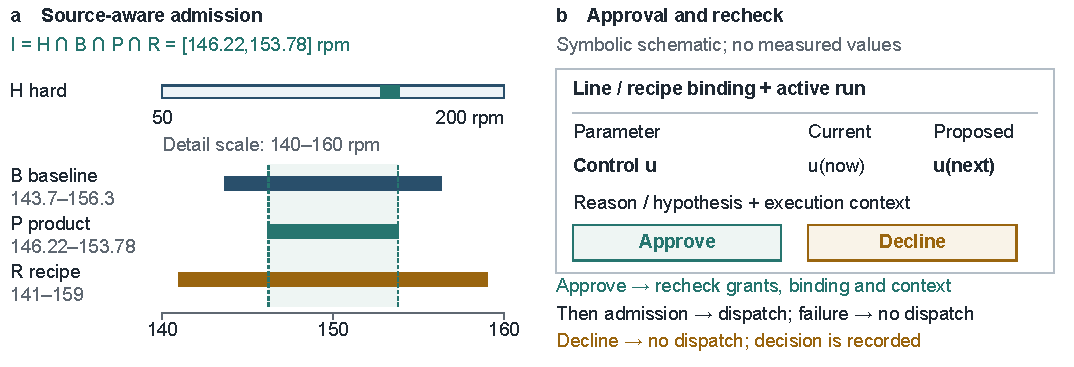
\includegraphics[width=\textwidth]{resources/fig-admission-hitl-2026.pdf}
\caption{Admission and approval boundaries. (a) Illustrative RPM
configuration, not experimental data: online node interventions use the
four-layer interval of Eq.~(\ref{eq:admission}), whereas recipe dispatch
omits the previous recipe window. (b) Symbolic human approval binds a
proposed action and its context tuple; execution rechecks the active
line--product--recipe--run context, authority, and applicable limits.
Approval does not reserve equipment state.}
\label{fig:hitl}
\end{figure*}

A \texttt{recipe\_trial} illustrates the operation sequence: the handler
checks the bound recipe, active run, candidate parameters, and route timing;
if required, it requests approval; after revalidation, it submits a bounded
batch through the configured driver and returns a per-parameter receipt.
The caller obtains later DAQ observations separately and may then update,
apply, or roll back a recipe. A trial neither saves nor applies a recipe
version. The driver registry maps semantic controls to configured protocol
drivers, keeping protocol details out of agent operation arguments.

Receipts and observations answer different questions. A command result is
graded as readback-verified, transport-acknowledged, or unverified; a
readback mismatch can trigger up to three reads at 2\,s intervals. Recipe
batches retain per-parameter verification outcomes. DAQ stores subsequent
timestamped process observations, while recipe versions, approvals, and
task records remain service-owned records linked where a route supplies the
corresponding identifiers. A verified setpoint confirms the command path,
not target attainment. This distinction defines the evidence chain evaluated
in Section~\ref{sec:eval}.


\section{Experimental Evaluation}
\label{sec:eval}
We evaluate route-specific record continuity across two configured scenes, one
blueprint-onboarding replay, a mock-state approval-context guard, and four
scripted scenario missions. Each study uses its own protocol and is reported
separately. All plant-facing tests use software simulators; no physical-plant
trial or independent process replication was performed.

\subsection{Test Design and Protocol}
\label{sec:eval-protocol}
The registered-task criterion is a linked task, approval, verified receipt,
and active-run sample. A direct call has no task record; it passes when its
receipt/readback and run-tagged sample are verified. The fixed-request replay
checks registered-harness route links without asserting task completion. The
context guard checks whether a changed line, product, recipe, or run is
refused before driver write.

We selected cast-film (OPC UA screw-speed command, MQTT thickness observation;
48--52\,$\mu$m target) and continuous annealing (Modbus TCP zone-3 setpoint
and strip-temperature observation; 700--760\,$^{\circ}$C target) to test the
same operation and record contract under different variable and protocol
mappings. The second scene checks route continuity after remapping; two scenes
do not establish support for unseen plants.
Across both scenes, the route study covered three caller routes: the
registered task harness, direct REST, and a fixture-backed command-line (CLI)
task. The registered-harness route had two execution conditions: six
model-mediated tasks and one scripted fixed-request replay per scene. The
model-mediated harness ran three sequential tasks per scene on one persistent
simulator; a hosted model selected each setting from a three-value
prevalidated set. The fixed-request replay, direct REST call, and CLI task
each ran once per scene in a separate isolated environment.
Each registered task had its own production and task context, while process
state persisted across the sequential tasks in its scene. After each operation
in all four execution conditions, the runner waited 20\,s, performed one explicit driver
probe, ingested the sample, and queried it by active-run ID. The registered
runner then checked task state; completion-to-sample latency was not recorded.
The fixed-request replay and CLI task used deterministic inputs; direct REST
did not invoke an external model.

The application's MQTT queue and Timescale service were unreachable in all
route-study runs, so each sample was a single explicit driver probe stored and
queried through the local SQLite fallback with online DAQ collection disabled;
the route results therefore assess invocation and application-record handling,
not the online DAQ pipeline. Direct REST created no task. All route-study
approvals were synthetic administrator decisions.

A separate onboarding replay used a fresh isolated application home and
the documented coating-line blueprint. It configured one Modbus/TCP device
with four setpoints and seven DAQ nodes, plus MES REST scalar, 48-point vector,
table, and image forms. Dedicated local MQTT and Timescale services were online
for DAQ checks; object storage was unavailable, so image artifacts used the
local-disk fallback. This was one configuration replay, not a route-study
trial.

The approval-context suite changed each field of the approved
line--product--recipe--run tuple for recipe apply, trial, and rollback with
dispatch enabled. A separate fault-injection case
changed context after asynchronous grant revalidation but before the caller's
final synchronous check. A test-only ablation removed only the tuple comparison
while retaining the other checks. These outcomes were recorded in mock-driver
state and are not process-level reliability estimates.

Finally, a deterministic mission script ran one seed-42 trajectory in each of
four simulators: injection molding, wastewater treatment, annealing, and
biaxially oriented polyethylene terephthalate (BOPET) film. Each mission
created its production context and channel, then issued controlled-operation
requests through the platform tool API. This protocol is
separate from the route-continuity study.
\subsection{Two-Scene Route Continuity}
\label{sec:testbed}
Table~\ref{tab:route-matrix} pairs each caller route or execution condition
with both scene mappings,
the resulting process samples, and the applicable record checks. The evidence
tests one shared execution contract under two configured mappings; it does not
establish route equivalence or support for unseen plants.

\begin{table*}[!t]
\centering
\caption{Caller-route coverage and one post-operation process sample per scene. In
each scene column, the requested setting is listed first and the measured
sample second. Samples were probed 20\,s after operation; all 12 were outside
their scene's target band.}
\label{tab:route-matrix}
\footnotesize
\setlength{\tabcolsep}{4pt}
\begin{tabularx}{\textwidth}{@{}>{\raggedright\arraybackslash}p{2.6cm}XX>{\raggedright\arraybackslash}p{5.2cm}@{}}
\toprule
Caller route / condition & \shortstack[l]{Cast film\\command / thickness sample\\(target: 48--52\,$\mu$m)} &
\shortstack[l]{Annealing\\setpoint / strip-temperature sample\\(target: 700--760\,$^{\circ}$C)} &
Verified route evidence \\
\midrule
Registered harness (model-mediated) &
\shortstack[l]{125/130/125\,rpm\\45.69/46.69/45.69\,$\mu$m} &
\shortstack[l]{745\,$^{\circ}$C each\\679.60/677.70/678.10\,$^{\circ}$C} &
All six tasks completed; task, approval, verified receipt, active run, and
sample links passed. \\
Registered harness (fixed-request replay) &
\shortstack[l]{125\,rpm\\46.37\,$\mu$m} &
\shortstack[l]{735\,$^{\circ}$C\\674.80\,$^{\circ}$C} &
Approval, receipt, and run-tagged sample links passed in both scenes; task
completion was not asserted. \\
Direct REST call &
\shortstack[l]{125\,rpm\\46.37\,$\mu$m} &
\shortstack[l]{735\,$^{\circ}$C\\675.20\,$^{\circ}$C} &
Verified receipt/readback and run-tagged sample in both scenes; no task record
was created. \\
Fixture-backed CLI task &
\shortstack[l]{125\,rpm\\46.38\,$\mu$m} &
\shortstack[l]{735\,$^{\circ}$C\\674.40\,$^{\circ}$C} &
Both tasks completed with linked approval, receipt, active run, and sample
records. \\
\bottomrule
\end{tabularx}
\end{table*}

All 12 route-study samples were below their scene target. Registered-task
pre-task readings were 55.82/45.69/46.69\,$\mu$m and
675.40/678.30/676.90\,$^{\circ}$C; five of six tasks began below target and
one cast-film task began above it. Process state carried across the sequential
tasks. One post-operation sample cannot show a response trajectory, steady
state, or setting quality, and samples from separate single-run paths do not
establish route equivalence.



\subsection{Blueprint-Driven Scenario Onboarding}
\label{sec:coating-onboarding}
One coating-line blueprint replay instantiated a Modbus/TCP device with four setpoints,
seven DAQ nodes, and four MES REST forms (scalar, vector, table, and image).
Connectivity preflight, provisioning, and channel construction completed
without failures; all forms returned the expected fields. Dedicated MQTT and
Timescale services supported DAQ checks; image artifacts used local-disk
fallback because object storage was unavailable. The verifier confirmed sample
availability, range rejection, legal write/readback, recipe mapping, channel
and plug-in checks, and zero writes to a protected line. A synthetic
automatic-approval smoke write changed line speed from 37 to 39 m/min within the
recipe window and was confirmed by the PLC twin. This single replay supports
the documented onboarding workflow only: profiles and bindings were not varied,
and the source commit was not pinned. It does not establish general portability,
repeatability, process attainment, film quality, human-review performance, or
physical transfer. Supplementary File S1 contains the replay evidence.
\subsection{Approval-Context Guard and Ablation}
\label{sec:guard-results}
The production handler blocked every injected one-field mutation before a mock
write or execution record. The queued context change was also refused before
\texttt{recipe\_apply} dispatch. In the ablation, removing the tuple comparison
allowed six product/run changes through; each produced two mock writes and an
execution record, while the other checks still blocked line/recipe changes.

The ablation isolates the tuple comparison within the tested software state.
It does not demonstrate atomicity during network or device I/O, safe physical
operation, operator effectiveness, or end-to-end DAQ integrity.

\subsection{Four-Scenario Control Sequences and Outcomes}
\label{sec:scenario-sequences}
The four-scenario campaign complements the route-continuity study with
scenario-specific control and process-response sequences. Fig.~\ref{fig:missions}
shows the four seed-42 simulator missions, one scripted trajectory per scenario.
Each column pairs operation requests with process-variable (PV) observations
and its own target window; event indices give order, not elapsed time.

\begin{figure*}[!t]
\centering
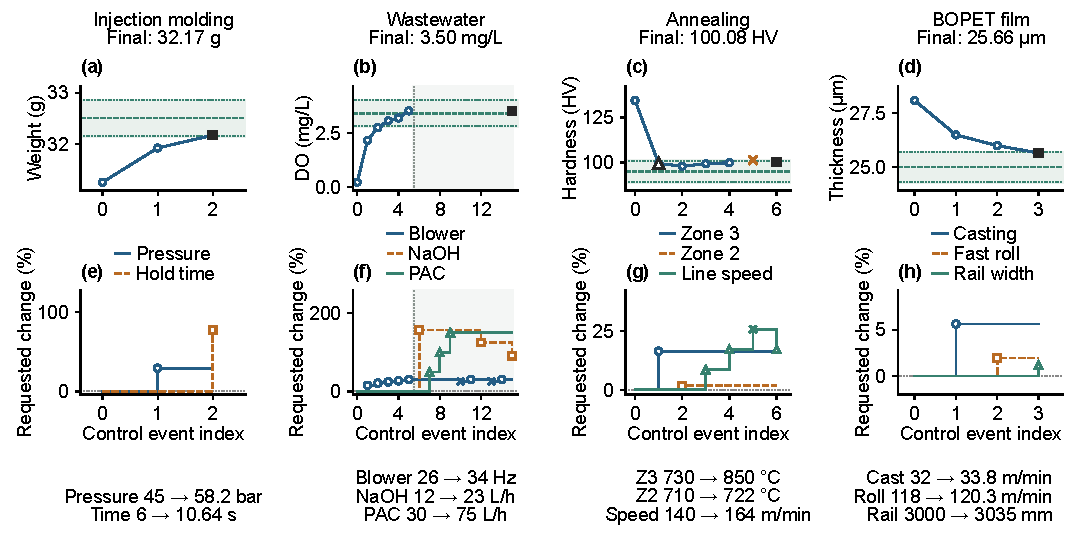
\includegraphics[width=\textwidth]{resources/fig-missions-controls.pdf}
\caption{Four-scenario simulator control sequences and outcomes (seed 42; one
scripted trajectory per scenario through the platform's governed operation
API). Upper panels show process-variable (PV) observations and scenario-specific
target windows; lower panels show requested setpoint changes from baseline.
Black squares mark mission-final readings; for injection molding and BOPET they
overlap the last observation.
In wastewater treatment, later sodium-hydroxide (NaOH) and polyaluminium-
chloride (PAC) requests belong to pH and total-phosphorus stages, and the
mission-final dissolved-oxygen (DO) reading (3.50\,mg/L) is not
joined to the last trajectory observation (3.517\,mg/L). Crosses mark reverted
requests. In annealing, Z3 and Z2 denote zone-3 and zone-2 temperature
setpoints. The open triangle marks the 99.46 Vickers-hardness (HV) event
without a linked optimization record; the cross is the
101.3-HV event-text value after a reverted 176\,m/min candidate, not a
structured
trajectory observation. Requests are not device readbacks. These scripted
scenario missions are separate from the route-continuity study and do not
establish route-level process performance or a common optimizer score.}
\label{fig:missions}
\end{figure*}

Injection-molding pressure and hold-time changes accompanied a weight increase
from 31.25 to 32.17\,g, within the $32.5\pm0.35$\,g window. Five wastewater
blower increments raised dissolved oxygen (DO) from 0.214 to 3.517\,mg/L,
within the $3.4\pm0.6$\,mg/L window; subsequent NaOH and polyaluminium
chloride (PAC) actions addressed separate pH and phosphorus stages. In
annealing, zone-3/zone-2 setpoints and line-speed changes preceded a terminal Vickers hardness of
100.08\,HV,
within the $95\pm6$\,HV window. Biaxially oriented polyethylene
terephthalate (BOPET) thickness fell from 28.10 to 25.66\,$\mu$m under the
plotted casting, roll-speed, and rail-width changes, within its
$25.0\pm0.7$\,$\mu$m window. Thus, each scripted mission reported a terminal
value in its scenario target window. Wastewater and annealing terminal values
differ from their final structured trajectory observations, as marked in
Fig.~\ref{fig:missions}. One trajectory per scene shows scenario-specific
feedback but does not establish repeatability or route-level process
attainment; the route and mission studies used different entry, controller,
and sampling protocols.
\subsection{Evidence Synthesis}
Across the studies, tested routes retained their applicable records across two
configured mappings, but all 12 route samples remained below target. The
blueprint replay completed one documented onboarding workflow and a confirmed
simulator write; the mock-state guard blocked injected stale contexts before
software dispatch. The four mission-terminal values fell within their
scenario-specific windows. These results support selected integration and
scenario-specific simulator behavior. Because entry and sampling protocols
differ, the process datasets are not pooled. Verified readback confirms the
command path, while the later sample records process status; neither establishes
route-level process attainment, repeatability, process improvement, general
portability, or physical-plant performance. Supplementary File S1 contains the
supporting evidence.

\section{Discussion}
\label{sec:limits}
This section interprets the results against the design contract and then states
what the evidence does not cover.

\subsection{Interpretation}
The implementation routes selected task and direct-call paths through a
shared named-operation boundary. Tests verify the applicable task, approval,
receipt, readback, and sample links across two different simulator mappings;
they do not establish route equivalence.

The blueprint replay adds protocol access, heterogeneous MES data, channel
construction, acquisition, and one approved simulator write. It was not
repeated with changed profiles or bindings, so it supports only the documented
blueprint workflow.

Route-study samples ranged from 45.69 to 46.69\,$\mu$m for cast film and
674.40 to 679.60\,$^{\circ}$C for annealing, all outside their target bands.
Each was a single probe 20\,s after an operation; pre-task values were already
out of band, so these readings establish neither a response curve nor
convergence.

The four-scenario campaign reports mission-terminal values inside the
scenario windows for injection molding, wastewater treatment, annealing, and
BOPET film. Each has one deterministic scripted trajectory; for wastewater
and annealing, the terminal mission value differs from the final structured
sample, as Fig.~5 marks. This shows scenario-specific feedback, not
repeatability or route-level process attainment.

This distinction is central to the framework: readback confirms that a
setpoint reached the configured device, while the later process sample records
whether the target was met. Keeping these as separate linked records avoids
equating command completion with product attainment. The tests validate this
reporting behavior, not improved control quality.

All route-study runs used SQLite fallback because MQTT and Timescale were
unavailable; they therefore do not validate the online DAQ pipeline. The
onboarding replay used
isolated online MQTT/Timescale services. Together, the tests cover two
configured route mappings and one separate blueprint-driven onboarding
workflow.

Under mock state, comparing the approved line--product--recipe--run tuple
blocked product/run mutations that the retained checks alone did not reject.
This is a software-dispatch result; synthetic approval does not measure human
review performance \cite{parasuramanmanzey2010complacency,parasuraman2000model,bainbridge1983ironies}.

\subsection{Scope and Limitations}
Only the reported adapters and scene configurations were exercised. The
single blueprint replay does not test repeated onboarding, profile/binding
reuse, unseen scenes, or physical transfer; the runs used working-tree builds without pinned
source commits. The study also lacks a platform baseline and does not establish
adapter interchangeability, online DAQ operation in route trials, or comparative
efficiency. Such claims require matched deployments and shared integration
effort or record-completeness measures.

The route study used three sequential tasks and one post-trial sample per task
on one simulator per scene; the four-scenario campaign used one trajectory per
scene. These are not independent replicates and cannot establish a response
curve or repeatability. Follow-up work should vary profiles, repeat trials
with pre/post measurements, and compare a defined alternative integration
path. Operation restrictions do not establish security
\cite{greshake2023injection,liu2024pinjection,iec62443-3-3} or replace
independent PLC/safety-instrumented system (SIS) safeguards \cite{iec61511}.

Scope and channel-policy refusals are not uniformly persisted; auditability
is limited to the records and denial classes described in Section~IV.

\section{Conclusion}
\label{sec:conclusion}
AgentWorkShop brings task adapters, production context, named operations,
semantic I/O, configured protocol drivers, and service-owned records into a
modular task-to-device framework. Tested task routes and direct calls used a
shared operation boundary across cast-film and annealing simulator mappings
while preserving route-specific records. A separate replay completed one
documented coating-line onboarding configuration with online DAQ checks and a
simulator-confirmed smoke write. A four-scenario simulator campaign recorded
scripted control sequences and mission-terminal values within scenario target
windows, while route-study samples remained below target. A mock-state ablation
isolated the effect of an approval-bound context check. The study establishes
selected integration, scenario-specific simulator behavior, one simulated
onboarding instance, and software-contract behavior; it does not establish
repeatability, route equivalence, process improvement, configuration reuse,
physical transfer, general portability, or comparative platform benefit.


\bibliographystyle{IEEEtran}
% Keep IEEEtran's default bibliography size and leading.
\bibliography{resources/refs}

\end{document}
